\section{问题一：油价预测与冲突影响识别}

\subsection{月度预测模型与评价口径}

油价具有接近随机游走、结构突变频繁和实时数据易修订的特点，复杂模型未必稳定优于
简单基线\cite{baumeister2012,baumeister2015}。本文以2010年1月至2019年12月为
初始训练段，自2020年1月起按月扩展窗口回测。预测期限固定为1、3、6个月，任一
目标月的训练样本截止于对应预测原点。基线no-change为

\begin{equation}
  \widehat{\ln P}_{t+h|t}^{\,NC}=\ln P_t.
  \label{eq:nochange}
\end{equation}

候选模型包括ARIMA、带滞后库存、美元和GPR的SARIMAX、阻尼趋势ETS、Theta
以及五者等权组合。以SARIMAX为例，模型写为

\begin{equation}
  \Phi(L)(1-L)\ln P_t
  =c+\boldsymbol{\beta}^{\mathsf T}X_{t-1}+\Theta(L)\varepsilon_t,
  \label{eq:sarimax}
\end{equation}

其中 $X_{t-1}$ 只含预测原点已知的月末库存、广义美元收益和GPR标准化值。ARIMA与
SARIMAX的 $p,q\in\{0,1,2\}$ 在初始训练集内按AIC选择，避免在测试集调参。

令 $e_{m,h,t}=\ln P_t-\widehat{\ln P}_{m,t|t-h}$，使用

\begin{equation}
  RMSE_{m,h}=\sqrt{\frac{1}{N_h}\sum_t e_{m,h,t}^{2}},\qquad
  RRMSE_{m,h}=\frac{RMSE_{m,h}}{RMSE_{NC,h}}
  \label{eq:forecastmetric}
\end{equation}

评价相对基线的误差。对模型与no-change的平方误差和绝对误差差序列进行
DM检验，并采用HLN小样本修正。若
$RRMSE>1.05$ 或显著劣于基线则判为失败；差异很小且不显著时判为条件可用，而不是
宣称复杂模型更优。

\begin{table}[H]
  \centering
  \small
  \caption{固定滚动回测下的代表性预测结果}
  \label{tab:q1-backtest}
  \begin{tabular}{cccccc}
    \toprule
    期限/月 & 模型 & RMSE & 相对RMSE & DM--HLN $p$ 值 & 状态 \\
    \midrule
    1 & no-change & 0.1408 & 1.000 & -- & 通过 \\
    1 & Theta & 0.1409 & 1.001 & 0.645 & 条件可用 \\
    1 & SARIMAX & 0.1442 & 1.025 & 0.830 & 条件可用 \\
    3 & no-change & 0.2660 & 1.000 & -- & 通过 \\
    3 & Theta & 0.2668 & 1.003 & 0.582 & 条件可用 \\
    6 & no-change & 0.3082 & 1.000 & -- & 通过 \\
    6 & Theta & 0.3105 & 1.007 & 0.570 & 条件可用 \\
    \bottomrule
  \end{tabular}
\end{table}

表\ref{tab:q1-backtest}表明三个期限均由no-change取得最低RMSE。这个结果反映
样本外油价的高噪声和结构突变，并非建模失败。以2026年2月均价70.887美元/桶为
原点，1、3、6月预测均为70.887美元/桶；其中2026年3月和5月实际均价分别为
103.135和107.140美元/桶，2026年8月尚未到期，只保留为预测值。图\ref{fig:q1-forecast}
展示一月期滚动预测，复杂模型没有形成稳定的误差优势。

\begin{figure}[H]
  \centering
  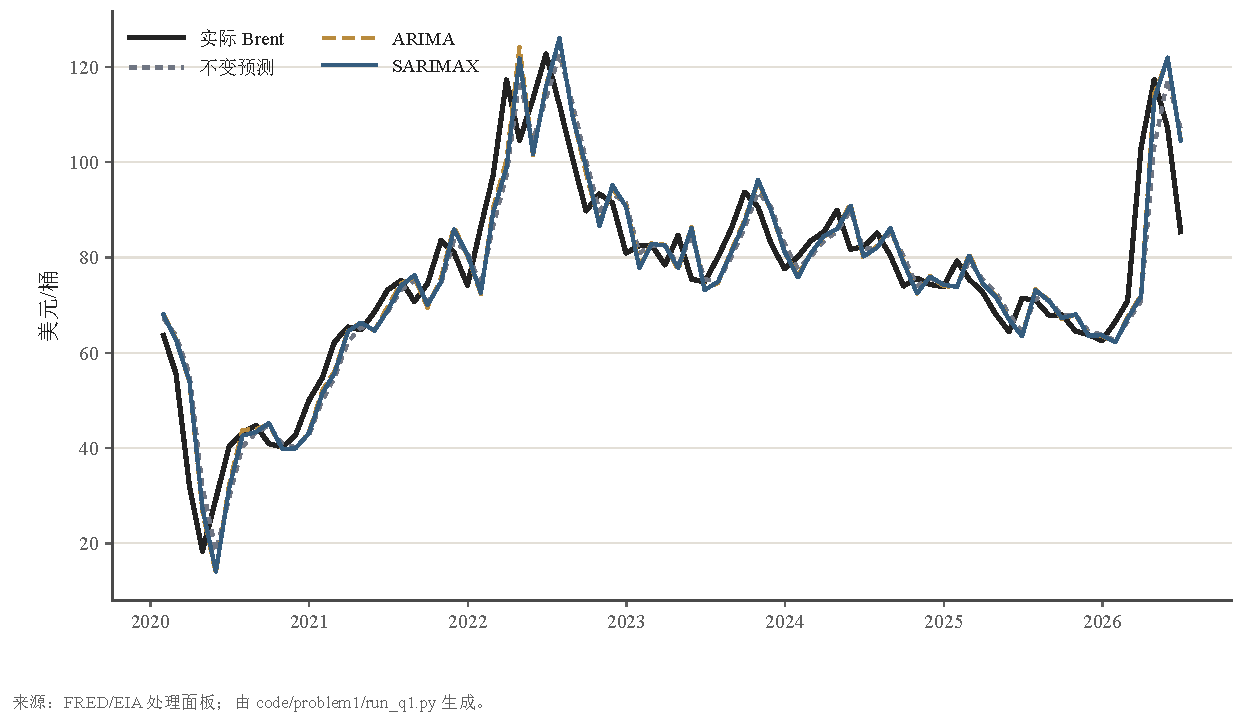
\includegraphics[width=0.90\textwidth]{../figures/q1_forecast_1m.pdf}
  \caption{Brent一月期扩展窗口预测与实际值}
  \label{fig:q1-forecast}
\end{figure}

\subsection{多阶段事件研究}

冲突日期与政策日期按表\ref{tab:event-timeline}分开编码。对2024年1月至事件前最后
交易日的Brent日收益拟合AR(3) 并控制广义美元收益，得到条件期望
$\widehat r_t^{,0}$。异常收益及累计异常收益定义为

\begin{equation}
  AR_t=r_t-\widehat r_t^{\,0},\qquad
  CAR[0,H]=\sum_{j=0}^{H}AR_{t_0+j},\quad H=0,1,2.
  \label{eq:car}
\end{equation}

为避免把单日常规标准误当作强因果证据，本文从非事件周末构造同口径伪事件。若 $B$
个安慰剂窗口中有 $b$ 个绝对CAR不小于真实事件，则经验显著性采用
$p_{emp}=(b+1)/(B+1)$，从而不会报告有限样本下不合理的零概率。

\begin{table}[H]
  \centering
  \small
  \caption{外部冲突、航运受阻、国内调控与缓和阶段时间线}
  \label{tab:event-timeline}
  \begin{tabularx}{0.97\textwidth}{p{0.13\textwidth}p{0.13\textwidth}p{0.20\textwidth}Xp{0.13\textwidth}}
    \toprule
    日期 & 编号 & 事件 & 主要通道 & 模型用途 \\
    \midrule
    2026-02-28 & E1 & 军事行动开始 & 供给中断风险、预防性需求与风险溢价 & 事件起点 \\
    2026-03-02 & E2 & 海峡运输受阻 & 实物流量、运价与保险成本 & 阶段变量 \\
    2026-03-23、04-07 & P1、P2 & 中国临时调控 & 降低当期国内价格传导 & 政策反事实 \\
    2026-06-17 & E3 & 通行恢复谅解 & 供应恢复预期与风险溢价回落 & 缓和阶段 \\
    \bottomrule
  \end{tabularx}
\end{table}

\begin{table}[H]
  \centering
  \small
  \caption{E1事件窗口的Brent累计异常收益}
  \label{tab:q1-car}
  \begin{tabular}{ccccc}
    \toprule
    窗口 & CAR & 常规95\% 区间 & 经验 $p$ 值 & 交易日数 \\
    \midrule
    $[0]$ & 0.0797 & $[0.0415,\,0.1178]$ & 0.0112 & 1 \\
    $[0,+1]$ & 0.1561 & $[0.1021,\,0.2101]$ & 0.0102 & 2 \\
    $[0,+2]$ & 0.1355 & $[0.0694,\,0.2016]$ & 0.0208 & 3 \\
    \bottomrule
  \end{tabular}
\end{table}

三组CAR均高于绝大多数匹配周末安慰剂，说明E1附近存在经济量级较大的事件相关
异常上涨。与此同时，战前模型递归生成的价格路径与实际价格之差记作

\begin{equation}
  ARBaselineGap_t=P_t-\widehat P_t^{\,AR\ baseline}.
  \label{eq:argap}
\end{equation}

该差额用于展示实际走势偏离战前自回归规律的程度；由于同期供需和其他新闻不能完全
排除，本文不将其称为``无战争价格''或战争净溢价。

\subsection{结构冲击与条件波动}

为给第二问提供具有经济含义的月度冲击，构造向量
$z_t=(\Delta q_t,a_t,\Delta p_t^{real})^{\mathsf T}$，分别表示全球液体燃料供给增长、
全球真实活动和实际Brent收益，并估计

\begin{equation}
  A(L)z_t=u_t,\qquad u_t=B\epsilon_t,
  \label{eq:svar}
\end{equation}

其中 $B$ 由Cholesky分解识别。BIC选出6阶稳定VAR，白噪声检验
$p=0.382$，三类结构冲击均有186个有效月。该分解遵循不同油价冲击不能混为一谈的
原则\cite{kilian2009}，但仍受递归排序约束。

日度波动采用战前样本拟合GJR--GARCH(1,1)：

\begin{equation}
  h_t=\omega+\alpha\varepsilon_{t-1}^{2}
  +\gamma I(\varepsilon_{t-1}<0)\varepsilon_{t-1}^{2}+\beta h_{t-1}.
  \label{eq:gjr}
\end{equation}

战前条件波动率中位数为1.743\%。E1即时窗口、E2航运受阻阶段和E3缓和阶段分别为
战前的1.587、2.214和1.566倍。可见波动压力在事实性运输受阻阶段最高，缓和后虽有
下降但尚未回到战前水平。该结果只描述金融市场波动，不能直接解释为实体经济损失。

\subsection{问题一小结}

预测层面，no-change在固定回测中诚实胜出；事件层面，E1三个交易日窗口的CAR及
安慰剂检验支持显著的事件相关异常上涨；机制层面，递归VAR输出供给、需求和石油特定
风险冲击，GJR--GARCH则显示航运受阻阶段条件波动最强。三类证据共同回答题意，但不把
预测误差、描述性基准差额或单次事件关联夸大为战争的严格净因果贡献。
